% Member 4 - Section 3.1 Overall Framework
\subsection{Overall Framework}
\label{sec:overall_framework}

Fig.~\ref{fig:framework} summarizes the pipeline. All three experimental groups share one architecture, one set of data splits, and one evaluation protocol, and differ in exactly one factor: the set of images used for training.

\begin{figure}[t]
\centering
% Overall framework diagram. Source: figures/framework.mmd (Mermaid).
% Render with:  npx -y @mermaid-js/mermaid-cli -i figures/framework.mmd -o figures/framework.pdf -b white -s 2
% If the PDF is absent, fall back to the PNG, and finally to a placeholder.
\IfFileExists{figures/framework.pdf}{%
  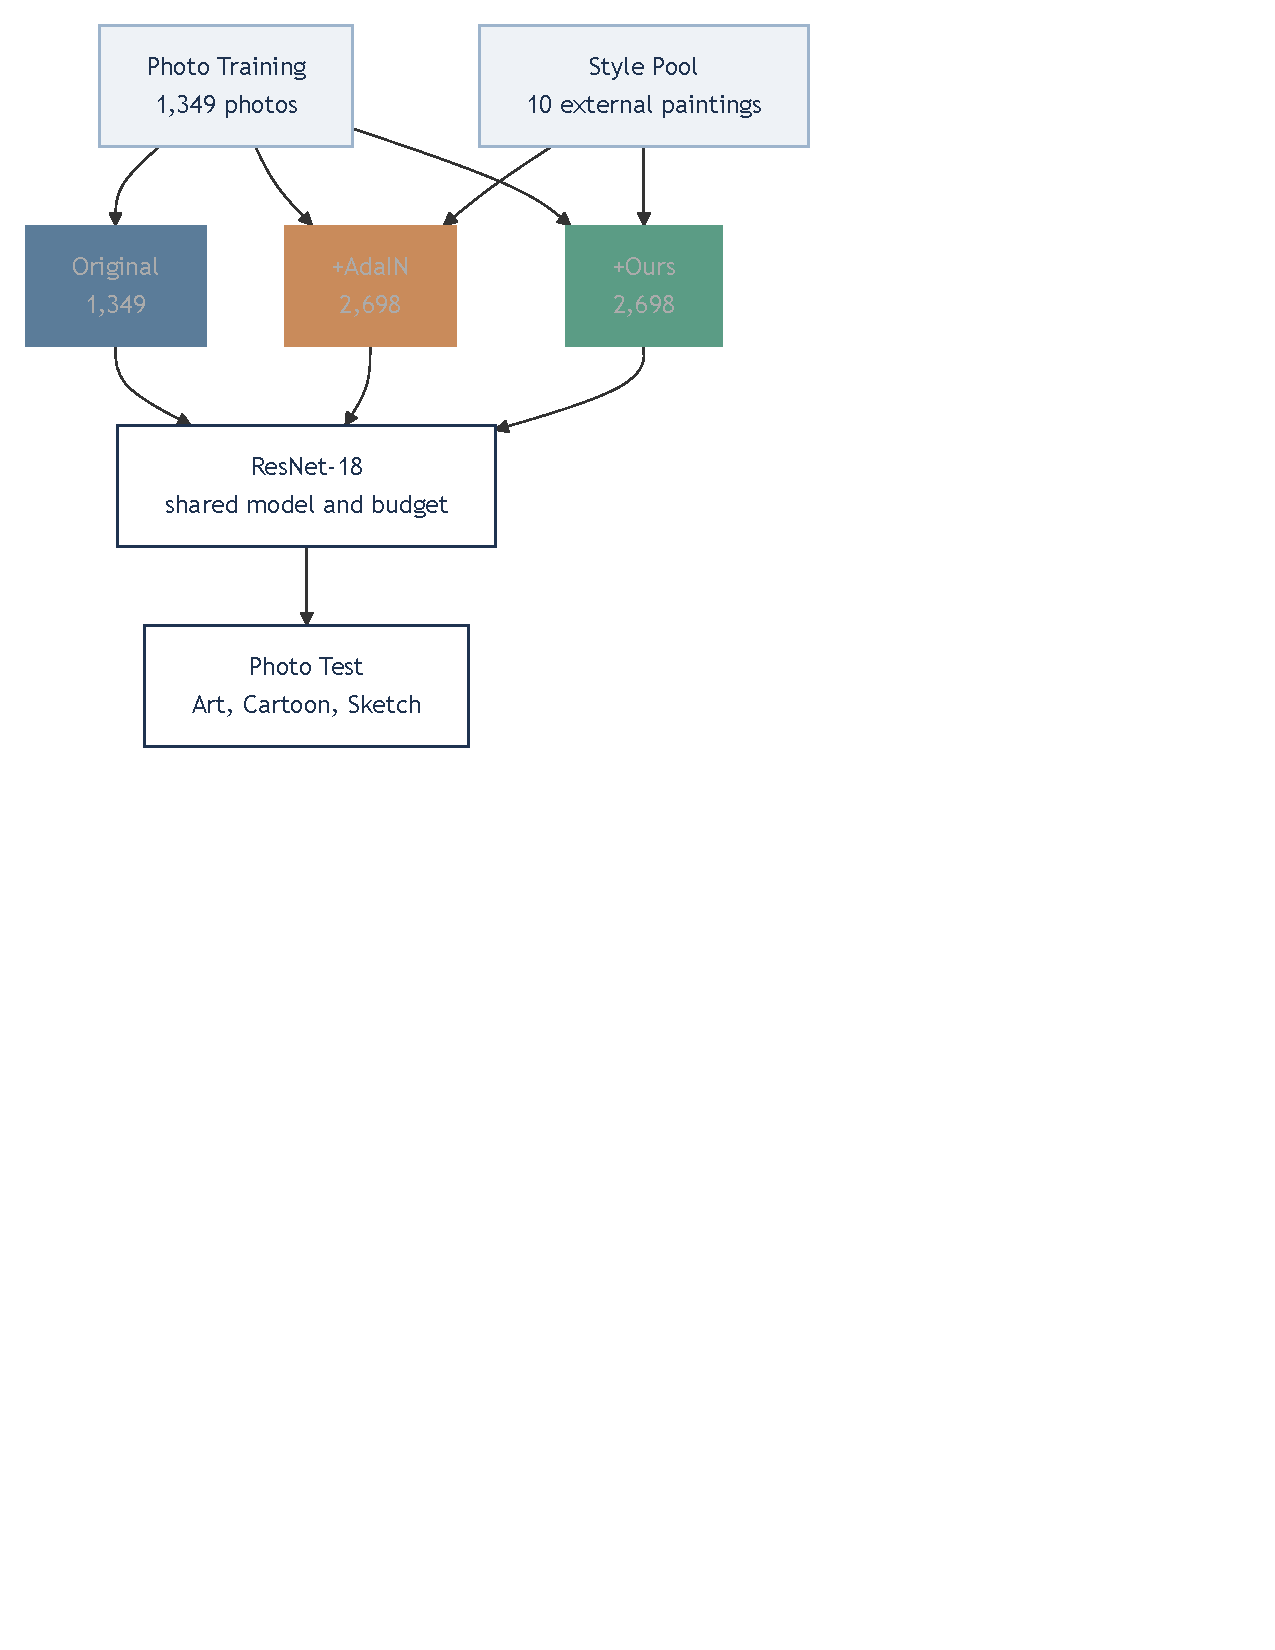
\includegraphics[width=\columnwidth]{figures/framework.pdf}%
}{%
  \IfFileExists{figures/framework.png}{%
    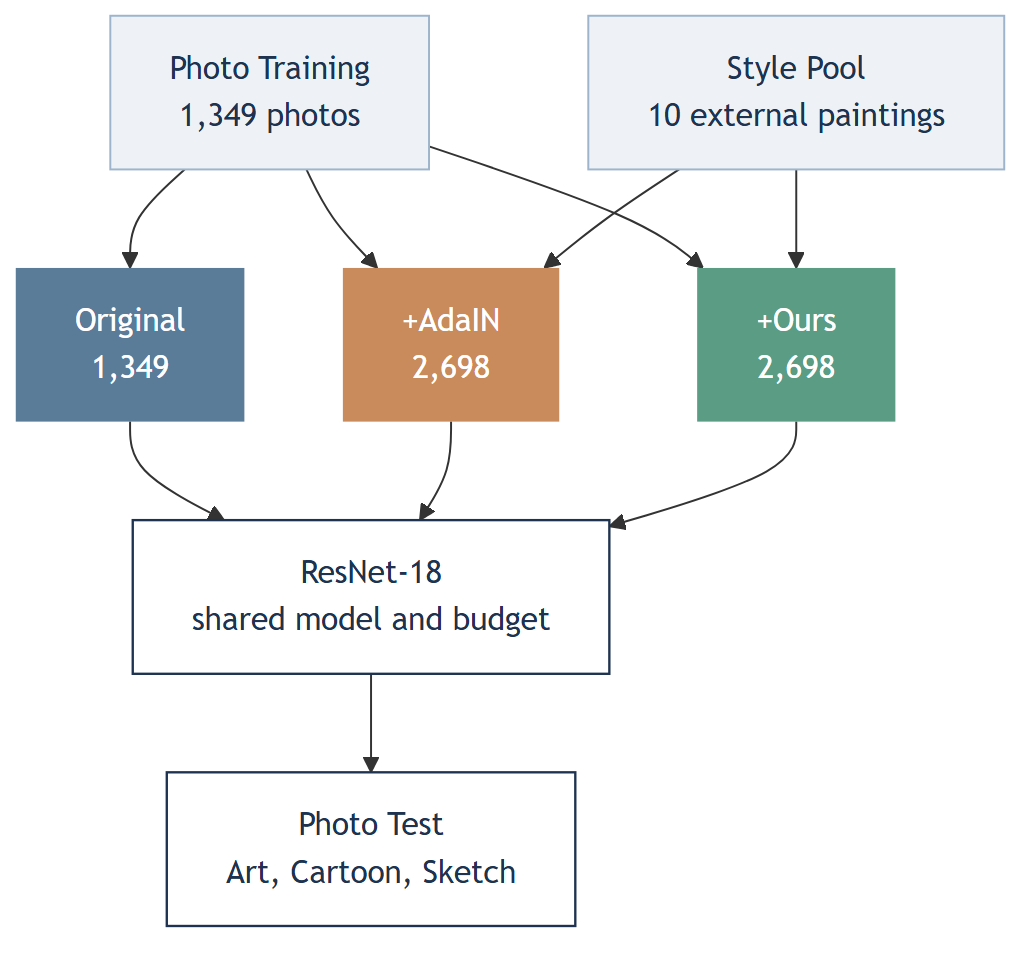
\includegraphics[width=\columnwidth]{figures/framework.png}%
  }{%
    \fbox{\parbox[c][2.2cm][c]{\dimexpr\columnwidth-2\fboxsep-2\fboxrule\relax}{\centering Placeholder: overall framework figure (planned).}}%
  }%
}
\caption{Overall framework. Photo Training images feed three training sets: originals only, originals plus AdaIN stylizations, and originals plus structure-preserving stylizations. Both stylized sets draw their style references from one frozen pool of external paintings. A single ResNet-18 training and evaluation protocol is applied to all three groups.}
\label{fig:framework}
\end{figure}

Stylized training images are produced \textit{offline}. Member 2's AdaIN generator and member 3's structure-preserving generator each write images to disk together with a manifest that records the content image, the style image, the style strength $\alpha$, and, for the structure-preserving variant, the structure parameter $\beta$. Training then reads from these fixed manifests, so the three groups go through an identical data-loading path. Nothing about the stylization is recomputed or resampled during classifier training, which keeps the classifier-side training code common to all groups.

Table~\ref{tab:groups} defines the three groups. The comparison Original vs.\ +AdaIN isolates the value of added style diversity (experiment 2), and +AdaIN vs.\ +Ours isolates the value of structure preservation (experiment 3), as detailed in Section~\ref{sec:exp_design}.

\begin{table}[t]
\caption{The three training groups. All groups use the same splits, model, and evaluation.}
\label{tab:groups}
\centering
\small
\setlength{\tabcolsep}{4pt}
\begin{tabular}{@{}lrr@{}}
\toprule
Group & Training images & Composition \\
\midrule
Original & 1{,}349 & Photo Training only \\
+AdaIN   & 2{,}698 & $+ 1{,}349$ AdaIN \\
+Ours    & 2{,}698 & $+ 1{,}349$ structure-preserving \\
\bottomrule
\end{tabular}
\end{table}
